%% Ein einfaches Template für einen Übungsbericht unter Verwendung des Hagenberg
%% Setups, basierend auf der LaTeX 'report' Standardklasse.
%%% äöüÄÖÜß  <-- keine deutschen Umlaute hier? UTF-faehigen Editor verwenden!

%%% Magic Comments zum Setzen der korrekten Parameter in kompatiblen IDEs
% !TeX encoding = utf8
% !TeX program = pdflatex
% !TeX spellcheck = de_DE
% !BIB program = biber

\documentclass[german,notitlepage,smartquotes]{hgbreport}
% Zulässige Optionen in [..]:
%    Hauptsprache: 'german' (default), 'english'
%    Option zur Umwandlung in typografische Anführungszeichen: 'smartquotes'
%    APA Zitierstil: 'apa'
%    Erzeuge keine separate Titelseite: 'notitlepage'
%%%-----------------------------------------------------------------------------

\RequirePackage[utf8]{inputenc} % bei Verw. von lualatex oder xelatex entfernen!
\usepackage{listings}

\renewcommand{\chapter}[1]{} % Deaktiviere den \chapter Befehl
\graphicspath{{images/}}     % Verzeichnis mit Bildern und Grafiken
\bibliography{references}    % Biblatex-Literaturdatei (references.bib)
\ExecuteBibliographyOptions{backref=false} % Keine Rückreferenzen bei Quellen

%%%-----------------------------------------------------------------------------
\setcounter{chapter}{1}	% <----- Auf die Übungsnummer setzen
%%%-----------------------------------------------------------------------------

\author{Julian Jany}                        % Name
\title{GP2 Generative Programmierung -- SS 2022\\ % Name der Übung
				Übungsabgabe \arabic{chapter}}
\date{\today}

%%%-----------------------------------------------------------------------------
\begin{document}
%%%-----------------------------------------------------------------------------
\maketitle
%%%-----------------------------------------------------------------------------

\begin{abstract}\noindent
\dots
\end{abstract}

%%%-----------------------------------------------------------------------------

\lstset{language=C++,
		basicstyle=\ttfamily\footnotesize,
		keywordstyle=\color{blue}\ttfamily,
		stringstyle=\color{red}\ttfamily,
		commentstyle=\color{green}\ttfamily,
		morecomment=[l][\color{magenta}]{\#}
}

\section{\dots like Bunnies}

\subsection{Code}

\lstinputlisting[caption=TMFs.h, language={[11]C++}]{src/Fibonacci/TMFs.h}
\lstinputlisting[caption=Fibonacci.h, language={[11]C++}]{src/Fibonacci/Fibonacci.h}
\lstinputlisting[caption=main.cpp, language={[11]C++}]{src/Fibonacci/main.cpp}

\subsection{Test}

\begin{figure}[h]
\centering
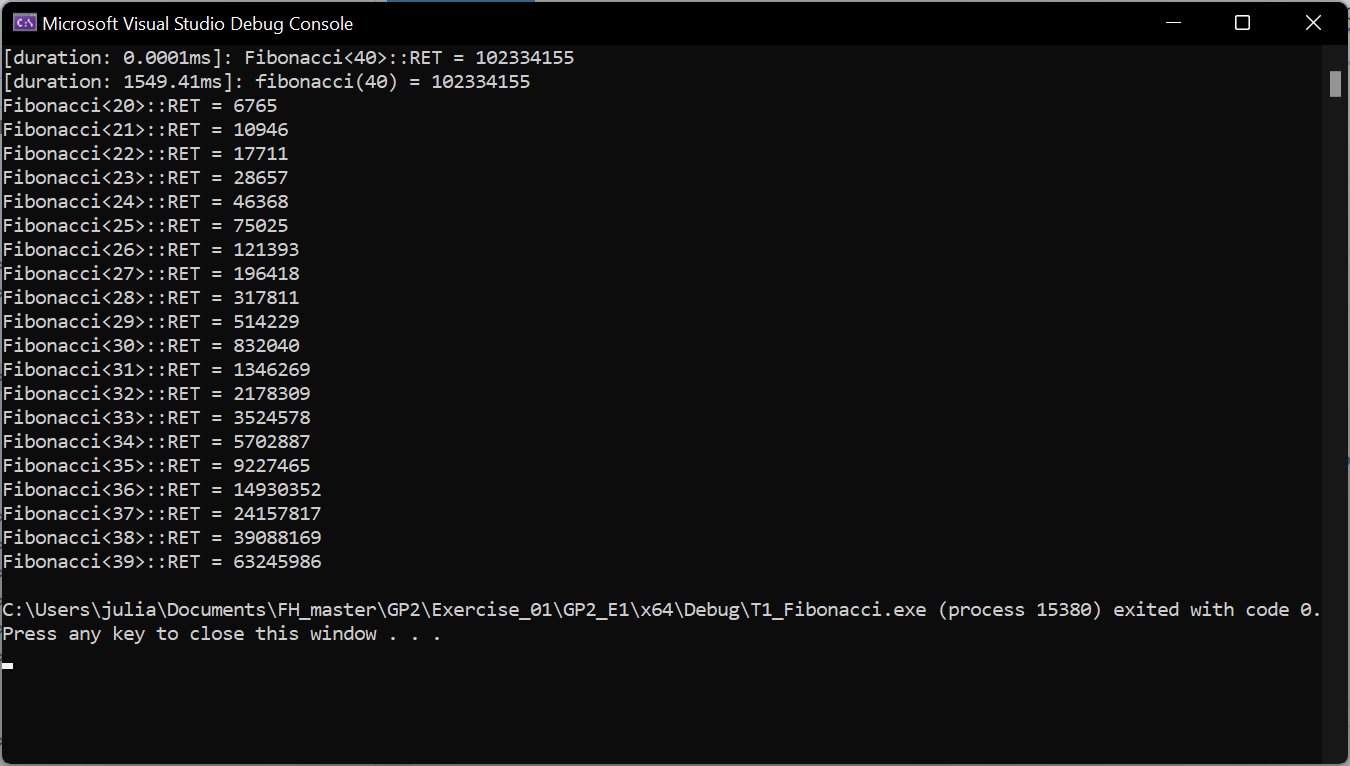
\includegraphics[width=.95\textwidth]{01_fib_test}
\caption{Testausgabe Fibonacci}
\label{fig:01_fib_test}
\end{figure}

%%%-----------------------------------------------------------------------------

\section{1, 2, 3, 4, 5, 6, 7, \dots}

\subsection{Lösungsidee}

\subsection{Code}

\subsection{Test}

%%%-----------------------------------------------------------------------------

\section{Counters off the Shelf}

\subsection{Lösungsidee}

\subsection{Code}

\subsection{Test}

%%%-----------------------------------------------------------------------------

\section*{Zusammenfassung und Anmerkungen}

%%%-----------------------------------------------------------------------------

% \section*{Quellen}

% \printbibliography[heading=noheader]

%%%-----------------------------------------------------------------------------
\end{document}
%%%-----------------------------------------------------------------------------